\documentclass[11pt]{article}
\usepackage[letterpaper,margin=1in]{geometry}
\usepackage{color}
\usepackage[dvipdfmx]{graphicx}
\usepackage{amsbsy}
\usepackage{amsmath}
\usepackage{adjustbox}
\usepackage{url}

\newcommand{\argmax}{\mathop{\rm arg~max}\limits}

\begin{document}
\title{Report on Assignment 1: K-nearest neighbors}
\author{Yoshinari Fujinuma}
\maketitle

\section{What is the relationship between the number of training examples and accuracy?}
The following graph shows the relationship between training examples and accuracy. The value of $k$ is fixed to $3$:
\begin{figure}[htb]
  %\begin{minipage}{0.5\hsize}
   \begin{center}
    \scalebox{0.5}
     {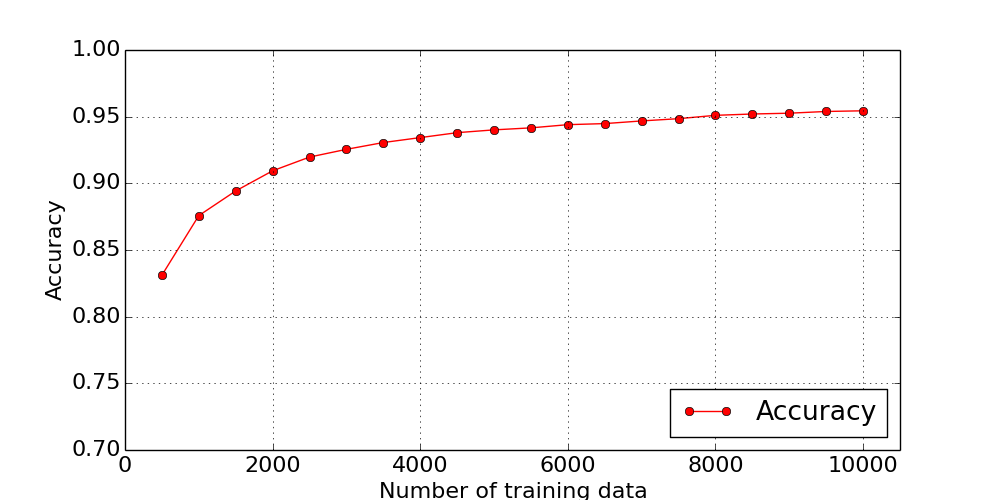
\includegraphics[]{figure_1.png}}
    \end{center}
    \caption{Segmentation results for katakana Twitter hashtags as a function of corpus size.}
    \label{fig:corpus_size}
  %\end{minipage}
%\vspace{0.1cm}
\end{figure}
\section{What is the relationship between $k$ and accuracy?}
The following graph shows the relationship between $k$ and accuracy
\section{What numbers get confused with each other most easily?}

\end{document}

